\chapter{Analysis of ORM frameworks}

We will start by exploring what Object-Relational Mappers (ORMs) are. We will introduce core concepts in relation to the .NET framework. After looking at modern trends and available ORMs, we will choose a representative sample. We will look at the candidates and analyze their features, strengths, and limitations. After we have a good theoretical understanding, we will practically verify capabilities and prepare performance benchmarks on a set of pre-selected queries. We will build upon this knowledge to design translation between different ORMs in the subsequent chapters.

\section{ORMs and important concepts}

We will briefly touch on how data is managed in .NET applications and how Object-Relational Mappers (ORMs) simplify this process.
At the most basic level, we can manually compose an SQL query, create a database connection, execute the query, and parse the results. We can achieve this with the help of standard .NET libraries, particularly ADO.NET. However, by directly using SQL, we introduce dependencies on a query language that lacks static typing in the context of C\#, forcing us to deal with raw strings. This can potentially lead to vulnerabilities, unnecessary dependencies, and additional complexity.

Nevertheless, ADO.NET remains crucial, and most .NET applications use it internally. Many ORM frameworks we will talk rely on it for communication with databases. We will briefly introduce ADO.NET and its core concepts.

To lower complexity related to database communication and data persistence, we use abstraction provided by ORMs. We will refer to those as ORMs or simply frameworks.

The level of abstraction varies depending on the specific framework. There are generally two categories, micro and macro ORMs. On one end of the spectrum, we have lightweight, usually performance-oriented frameworks. They offer a narrow set of features, some simple abstraction over ADO.NET. Some of those might not even be full ORMs, omitting the "relational" part entirely, as is the case with Dapper\cite{Dapper}. On the opposite end, we have full-fledged frameworks that completely abstract away database communication, providing abstraction over SQL and an extensive set of features to simplify the work of developers. \cite{Dapper}

\subsection{ADO.NET}
"ADO.NET provides consistent access to data sources such as SQL Server and XML" \cite{ADONET}. It provides components and models for connecting to those sources, executing commands, and retrieving results. All this functionality is built into \texttt{System.Data} library.

Let us look at a concrete code example, taken from Microsoft documentation \cite{ADONET}, adapted and shortened for the purposes of this text.
We can see the usage of key ADO.NET objects here, namely \texttt{SqlConnection}, \texttt{SqlCommand} and \texttt{SqlDataReader}. Managing the connection, building the query command and reading introduces a fair amount of overhead and manual control. The indexed access to \texttt{SqlDataReader} inside the \texttt{while} loop can end up being error-prone and increase the rosk of runtime exceptions. 

\begin{lstlisting}[language=CSharp]
const string connectionString = "...";

const string queryString =
    "SELECT ProductID, UnitPrice, ProductName from dbo.products "
    + "WHERE UnitPrice > @pricePoint "
    + "ORDER BY UnitPrice DESC;";

const int paramValue = 5;

using (SqlConnection connection = new(connectionString))
{
    SqlCommand command = new(queryString, connection);
    command.Parameters.AddWithValue("@pricePoint", paramValue);

    connection.Open();
    SqlDataReader reader = command.ExecuteReader();
    while (reader.Read())
    {
        Console.WriteLine($"{reader[0]}\t{reader[1]} ...");
    }
    reader.Close();
}
\end{lstlisting}

Although this approach is functional, it highlights why abstractions like ORMs are more desirable and popular.

\subsection{Entities and mapping}

TODO: briefly explain entities and mapping
- entity, domain model,
- mapping to tables

\subsection{Querying}

TODO: explain querying based on entities
- introduce LINQ as an alternative to SQL
- difference query vs method LINQ

\section{Selection process}
Now that we know the basic concepts of ORMs, we can move on to the criteria for selecting specific frameworks for our evaluation.

Important factors will be popularity and community support. Those can be estimated from the number of downloads on the .NET package manager NuGet\footnote{\url{https://www.nuget.org/}} or activity on GitHub\footnote{\url{https://github.com/}}. Since not all software is open source, we will limit ourselves to frameworks that are. We also  exclude outdated ORMs. Selected ones must have received at least some form of update or security fix in recent years.

Support for recent .NET versions is another essential factor. The versioning history of .NET is somewhat complicated. The original implementation, .NET Framework, was Windows-only and went up to version 4.8.1. Around 2016, Microsoft performed a major rework, focusing on cross-platform implementation. With a new name .NET Core, they started again at version 1.0. After .NET Core 3.1, the "Core" naming was dropped, and versions continued as .NET 5, .NET 6 and so on. Today, developing new applications using .NET Framework is not recommended, as it only receives security patches. The current long term support version is .NET 8, while .NET 9 is a standard term support release. In this text, we refer to the legacy platform as ".NET Framework" and to the new one as ".NET Core" or simply ".NET". \cite{NETFrameworkVersions}\cite{NETversions}

Another version to be aware of is .NET Standard. It is a formal API specification designed to unify .NET implementations. It allows libraries to be compatible with both .NET Framework and Core by targeting a common subset of APIs. However, this can restrict access to newer features and optimizations. \cite{NETStandard}

This work will be limited to ORMs supporting Microsoft SQL Server. As we will see, this is not a restrictive requirement. All major .NET ORMs offer SQL Server support.

Our goal is to select a representative and diverse sample for comparison and testing. We aim to include at least two of micro and macro ORM frameworks. We will also add frameworks with notably interesting capabilities.

\autoref{tab:orm-docs} lists all notable considered .NET ORM frameworks with a link to their homepage or repository.

\begin{table}[h]
\definecolor{lightgreen}{RGB}{217, 234, 211}
\centering
\begin{tabular}{|l|l|}
\hline
\textbf{ORM} & \textbf{URL} \\
\hline
\cellcolor{lightgreen}Dapper & \url{https://github.com/DapperLib/Dapper} \\
\cellcolor{lightgreen}Entity Framework 6 & \url{https://learn.microsoft.com/en-us/ef/ef6/} \\
\cellcolor{lightgreen}Entity Framework Core & \url{https://learn.microsoft.com/en-us/ef/core/} \\
\cellcolor{lightgreen}LINQ to DB (linq2db) & \url{https://linq2db.github.io/} \\
Massive & \url{https://github.com/FransBouma/Massive} \\
Mighty & \url{https://github.com/MightyOrm/Mighty} \\
\cellcolor{lightgreen}NHibernate & \url{https://nhibernate.info/} \\
Norm.NET & \url{https://vb-consulting.github.io/norm.net/} \\
\cellcolor{lightgreen}PetaPoco & \url{https://github.com/CollaboratingPlatypus/PetaPoco} \\
\cellcolor{lightgreen}RepoDB & \url{https://repodb.net/} \\
SqlMarshal & \url{https://github.com/kant2002/SqlMarshal} \\
XPO & \url{https://devexpress.com/Products/NET/ORM/} \\
\hline
\end{tabular}
\caption{Considered ORMs with selected ones highlighted in green\label{tab:orm-docs}}
\end{table}

XPO was not considered due to not being open source. The other excluded frameworks were found to be outdated or inactive. This was primarily determined by the lack of recent GitHub commits and low community engagement, such as star count. 

The final selection includes seven ORMs. The obvious choices were \textbf{Dapper}, \textbf{NHibernate} and \textbf{Entity Framework Core}, as they are the most widely used. We also include \textbf{Entity Framework 6} for completeness --- despite being older, it remains widely spread among legacy projects and meaningfully differs from EF Core, particularly in version compatibility. For the micro category, we selected \textbf{PetaPoco} to oppose Dapper. During our research, we also encountered frameworks that fall somewhere between micro and macro, offering some abstraction without the full complexity of macro ORMs. \textbf{LINQ to DB} extensively supports LINQ but stays lightweight. And \textbf{RepoDB} promises to be "easiest-to-use"\cite{RepoDB}. We will look into each ORM in detail and explore its capabilities in the next section.

\section{Feature comparison}
We will first introduce the methodology of our comparison, deciding what properties and information to look for. Then we will follow with an overview of each framework, finishing with an overall comparison.

We will start with gathering sources for each ORM, that includes links to documentation, repository, and a NuGet distribution. We will continue with a brief introduction, mainly based on what each framework's documentation or repository README file promises. We will follow with distribution, licensing, and version info. To get an idea of relevancy, we will check development cycles, community forums, and tool support. Then we will move onto more technical areas. We are interested in database system support and configuration, as well as how each ORM handles entity mapping and various aspects of database operations. And finally, we will compare our findings with initial promises and discuss best use cases.

\subsection{Dapper}\label{sec:feat_dapper}

Dapper~\cite{Dapper,DapperRepo} is an open-source micro ORM framework for .NET, originally developed by the team at Stack Overflow. It was created in response to the inefficiencies observed with LINQ to SQL -- an ORM that preceded the Entity Framework -- particularly under increasing traffic loads. Designed for performance and simplicity, Dapper functions as a lightweight wrapper around ADO.NET\footnote{\url{https://learn.microsoft.com/en-gb/dotnet/framework/data/adonet/}}, extending the \texttt{DbConnection} object with a set of additional methods to facilitate object mapping. Its primary focus lies in mapping SQL query results to .NET objects, and it does not offer built-in support for modelling relationships or managing database schemas.

The core strength of Dapper lies in its minimal abstraction and high execution speed. Developers retain full control over SQL queries, which allows precise use of SQL dialect features specific to a given database system. Dapper is compatible with all database engines supported by ADO.NET, including Microsoft SQL Server\footnote{\url{https://www.microsoft.com/en-gb/sql-server}}, Oracle\footnote{\url{https://www.oracle.com/database/}}, PostgreSQL\footnote{\url{https://www.postgresql.org/}}, and SQLite\footnote{\url{https://sqlite.org/}}. However, it delegates schema management entirely to the developer, as it does not provide mechanisms for schema versioning or migrations. Consequently, any changes to the database schema must be manually reflected in the SQL queries and the corresponding C\# entities.

Entity mapping in Dapper is handled by matching the names of query result columns with the properties of a specified .NET class. Only exact name matches are recognized, and aliases or naming conventions are not supported without relying on unofficial extensions. Relationships between entities are not automatically resolved, though the framework offers helper methods that enable manual mapping of joined queries using lambda expressions. This process still entails a non-negligible performance overhead and potential duplication, making it a practical but suboptimal alternative to proper relationship management. Moreover, Dapper does not support collection mapping or advanced data format serialization such as JSON or XML, unless the underlying SQL engine supports it natively and the developer writes custom SQL logic to handle it.

\begin{example}
\small
This code example\cite{DapperRepo} showcases an entity and a query returning one instance. Properties are matched and filled by names, the rest remain empty.

\begin{lstlisting}[language=CSharp]
public class Dog
{
    public int? Age { get; set; }
    public Guid Id { get; set; }
    public string Name { get; set; }
    public float? Weight { get; set; }

    public int IgnoredProperty { get { return 1; } }
}

var guid = Guid.NewGuid();
var dog = connection.Query<Dog>("select Age = @Age, Id = @Id", new { Age = (int?)null, Id = guid });
\end{lstlisting}
\qed
\end{example}

\begin{example}
\small
In this example, each post is connected to its owner. The lambda function in \texttt{Query} methods specifies how to connect the entities. Users are likely duplicated for each post. Overall, this is just a simplification of manual handling of the data, and overhead is still present. Real use cases could be more complex and inefficient.

\begin{lstlisting}[language=CSharp]
var sql =
@"select * from #Posts p
left join #Users u on u.Id = p.OwnerId
Order by p.Id";

var data = connection.Query<Post, User, Post>(
    sql, (post, user) => { post.Owner = user; return post;});
var post = data.First();
\end{lstlisting}
\qed
\end{example}

Dapper does not include capabilities such as change tracking, data seeding, or query logging. Batch operations are supported natively, while bulk operations require the use of a commercial extension (Dapper Plus)\footnote{\url{https://dapper-plus.net/}}. Transaction handling is available indirectly through ADO.NET or via community-supported extensions. All major methods have asynchronous counterparts, ensuring compatibility with modern asynchronous programming models in .NET. Despite the lack of official development tools, Dapper benefits from a variety of extensions, both official and community-driven. Notable examples include \texttt{Dapper.SqlBuilder}\footnote{\url{https://github.com/DapperLib/Dapper/tree/main/Dapper.SqlBuilder}} for SQL generation, \texttt{Dapper.Rainbow}\footnote{\url{https://github.com/DapperLib/Dapper/tree/main/Dapper.Rainbow}} for simplified CRUD operations, and \texttt{Dapper.EntityFramework}\footnote{\url{https://github.com/DapperLib/Dapper/tree/main/Dapper.EntityFramework}} for integrating with Entity Framework -- although the latter remains largely undocumented.

The project is distributed under the Apache 2.0 License\footnote{\url{https://github.com/DapperLib/Dapper/blob/main/License.txt}} and is freely available via GitHub\footnote{\url{https://github.com/DapperLib/Dapper}} and NuGet\footnote{\url{https://www.nuget.org/packages/dapper/}}. As of the latest release (version 2.1.66 in February 2025), Dapper has amassed over 395 million total downloads, with 120 million downloads in the past year alone\footnote{\url{TODO...}}. While the release cycle is not fixed, updates follow semantic versioning and are typically introduced in response to patches or new feature demands. The framework supports multiple .NET versions, including .NET Framework, .NET Standard, and .NET~8.

In terms of community support, Dapper exhibits a healthy level of maintenance with active issue tracking and contributions. Although responses to GitHub issues may be delayed, many questions receive attention either from maintainers or the broader community, including the original authors. Documentation is primarily hosted on an external website, Learn Dapper\footnote{\url{https://www.learndapper.com/}}, which is maintained by a sponsor responsible for developing the commercial extension Dapper Plus.

\begin{table}[H]
\centering
\caption{Comparison overview of ORM framework: Dapper}
\begin{tabular}{|l|l|}
\toprule
\textbf{Property} & \textbf{Dapper} \\
\midrule
\textbf{Type} & Micro ORM for .NET \\
\textbf{License} & Apache 2.0 \\
\textbf{Cost} & Free; Dapper Plus extension costs \$999/year/developer \\
\textbf{Sources} & \url{https://github.com/DapperLib/Dapper}, \url{https://www.nuget.org/packages/Dapper}, \url{https://www.learndapper.com} \\
\textbf{Latest version} & 2.1.66 (February 2025) \\
\textbf{Supported .NET} & .NET Framework, .NET Standard, .NET 8 \\
\textbf{ORM features} & Object mapping only; no relationship or collection support \\
\textbf{Query support} & Raw SQL; any dialect via ADO.NET; no LINQ support \\
\textbf{Mapping} & Maps result columns to entity properties by exact name; no aliases or conventions \\
\textbf{Relationship mapping} & Not supported directly; JOINs and result splitting possible manually \\
\textbf{Schema handling} & No migrations; schema defined in DB; SQL must be adjusted manually \\
\textbf{Change tracking} & Not supported \\
\textbf{Data seeding} & Not supported \\
\textbf{Query logging} & Not supported \\
\textbf{Transactions} & Supported via ADO.NET; extensions available \\
\textbf{Bulk operations} & Requires paid extension \\
\textbf{Async support} & Fully supported \\
\textbf{Caching} & Entity mapping cached internally; no data caching \\
\textbf{Community} & Maintained actively on GitHub; many questions on Stack Overflow, often answered by the author \\
\textbf{Documentation} & External site (Learn Dapper), maintained by extension sponsor; repository includes tests and examples \\
\textbf{Extensions (official)} & Dapper.SqlBuilder, Dapper.Rainbow, Dapper.EntityFramework \\
\textbf{Extensions (community)} & Dapper Plus (paid), Dapper.Transaction \\
\textbf{Tooling} & None available \\
\textbf{Supported databases} & All ADO.NET-compatible DBs: SQL Server, Oracle, SQLite, PostgreSQL, etc. \\
\textbf{Ideal use cases} & High-performance data reading, performance bottleneck zones, apps requiring full SQL control \\
\bottomrule
\end{tabular}
\end{table}

\subsection{PetaPoco}\label{sec:feat_petapoco}

PetaPoco\cite{PetaPoco} is our second chosen micro ORM. Although it changed recently --- it used to have a single-file code base with no dependencies. It is focused on performance and simplicity. Internally it uses ADO.NET like Dapper, yet it provides its own abstractions over it. The framework is configurable through a builder, resulting in \texttt{IDatabase} interface, on which methods are called. With a focus on mapping query results to objects, it does not provide any support for relationships. It provides full control over SQL with an inbuilt SQL builder to make composing it easier. 

Its small feature set and zero dependencies enable compatibility with a wide selection of database systems, including Microsoft SQL Server, MS Access\footnote{\url{https://support.microsoft.com/en-us/access}}, SQLite, MySQL\footnote{\url{https://www.mysql.com/}}, MariaDB\footnote{\url{https://mariadb.org/}}, and Oracle. Schema management is left to the developer. Templates for entity generation out of a database schema were provided, but were deprecated in the last major version.

Entity mapping supports automatic configuration through naming conventions---such as pluralizing property names to match database columns. A limited set of mapping attributes is offered. These can be used to map table and column names, primary keys, and ignore class properties. Like Dapper, it does not automatically handle relationships but provides helper methods for manual JOINs management.

\begin{example}
\small
In the following example, the table name and primary key are explicitly defined using attributes, while other properties rely on automatic mapping. The use of the SQL query builder is demonstrated. The projection and source table components in the query builder can be omitted when they can be inferred from the source entity.

\begin{lstlisting}[language=CSharp]
using PetaPoco;

[TableName("Sales.OrderLines")]
[PrimaryKey("OrderLineID")]
public class OrderLine
{
    public int OrderID { get; set; }
    public int OrderLineID { get; set; }
    public decimal? UnitPrice { get; set; }
}

decimal unitPrice = 25m;
var orderLines = db.Fetch<OrderLine>(
    Sql.Builder.Where("UnitPrice = @0", unitPrice)
);
\end{lstlisting}
\qed
\end{example}

No support for advanced data formats of collections is provided, with the exception of writing native SQL that can work with these structures. LINQ is not supported. Unofficial extension \texttt{StaTypPocoQueries.PetaPoco}\footnote{\url{https://github.com/asherber/StaTypPocoQueries.PetaPoco}} provides result modification methods such as \texttt{First}, \texttt{Single}, \texttt{Page}, and \texttt{Delete} with some selection capabilities. For data manipulation operations (DML), strongly-typed methods like \texttt{Insert}, \texttt{Save}, \texttt{Update}, and \texttt{Delete} are provided. 

Queries executed by the framework can be inspected during debugging. Transactions are supported, including nested transactions if the underlying database system allows. However, bulk operations are not available. Asynchronous versions of all methods are also provided. Advanced capabilities such as versioning, change tracking, and data seeding are not provided. The only notable extension is an unofficial \texttt{PetaPoco.SqlKata}\footnote{\url{https://github.com/asherber/PetaPoco.SqlKata}}, which is a more extensive SQL builder than the native one.

The library is distributed under the Apache 2.0 License\footnote{\url{https://github.com/CollaboratingPlatypus/PetaPoco/blob/development/LICENSE.txt}} and is open-sourced on GitHub\footnote{\url{https://github.com/CollaboratingPlatypus/PetaPoco}} and NuGet\footnote{\url{https://www.nuget.org/packages/PetaPoco.Compiled/}}. PetaPoco was downloaded 1.3 million times in total, with half a million in the last year. PetaPoco has been stagnating on major version 6 (6.0.683 in September 2024) for the past few years, with minor patches being done every few months in response to security patches or new feature demands. The library targets .NET Framework and Standard.

This ORM does not benefit from an extensive community support, with the only extensive source of information being its GitHub wiki\footnote{\url{https://github.com/CollaboratingPlatypus/PetaPoco/wiki}}. Integration tests for most database systems are available and could be used for reference.


\begin{table}[H]
\centering
\caption{Comparison overview of ORM framework: PetaPoco}
\begin{tabular}{|l|l|}
\toprule
\textbf{Property} & \textbf{PetaPoco} \\
\midrule
\textbf{Type} & Micro ORM for .NET \\
\textbf{License} & Apache 2.0 \\
\textbf{Cost} & Free \\
\textbf{Sources} & \url{https://github.com/CollaboratingPlatypus/PetaPoco}, \url{https://www.nuget.org/packages/PetaPoco.Compiled}  \\
\textbf{Latest version} & 6.0.683 (September 2024) \\
\textbf{Supported .NET} & .NET Framework, .NET Standard \\
\textbf{ORM features} & Object mapping only; no relationship or collection support \\
\textbf{Query support} & Raw SQL; wide DB support; limited LINQ through extension \\
\textbf{Mapping} & Maps automatically by exact name; conventions and some attributed available \\
\textbf{Relationship mapping} & Not supported directly; JOINs and result splitting possible manually \\
\textbf{Schema handling} & No migrations; schema defined in DB; SQL must be adjusted manually \\
\textbf{Change tracking} & Not supported \\
\textbf{Data seeding} & Not supported \\
\textbf{Query logging} & Accessible while debugging \\
\textbf{Transactions} & Supported; with nesting \\
\textbf{Bulk operations} & Not supported \\
\textbf{Async support} & Fully supported \\
\textbf{Caching} & No caching \\
\textbf{Community} & Maintained actively on GitHub; questions and issues not frequently responded to \\
\textbf{Documentation} & GitHub wiki; repository includes integration and unit tests\\
\textbf{Extensions (official)} & None \\
\textbf{Extensions (community)} & PetaPoco.SqlKata, StaTypPocoQueries.PetaPoco \\
\textbf{Tooling} & None available \\
\textbf{Supported databases} & Microsoft SQL Server, MS Access, SQLite, MySQL, MariaDB, Oracle, etc. \\
\textbf{Ideal use cases} & High-performance data reading, performance bottleneck zones, apps requiring full SQL control \\
\bottomrule
\end{tabular}
\end{table}



\subsection{RepoDB}

\subsection{LINQ to DB}

\subsection{NHibernate}
\subsection{EF Core}
\subsection{EF 6}

\section{Performance evaluation}\label{sec:perf_eval}

This chapter presents an experimental comparison of the seven selected ORM frameworks. 
The primary goals are to assert the correctness of our previous comparison, measure performance, and assess how effectively each framework integrates into the .NET through its supported query language.

For each framework, we will create a set of unit tests performing pre-selected queries. They should cover different areas of querying through ORMs, such as entity mapping, relationships, result modification, and aggregation.

We will only test read (SELECT) queries. Those cover a sufficiently large area of features and provide us with enough information to get some insight on capabilities and performance. Other non-read operations, including insert, update, and delete queries, could be explored in future work.

\subsection{Dataset and database}\label{sec:dataset_database}
% https://learn.microsoft.com/en-us/sql/samples/wide-world-importers-what-is?view=sql-server-ver16
To adequately test performance, we need a sufficiently large data set. Microsoft offers pre-made open source datasets.
For this comparison, the Wide World Importers sample database \cite{microsoftWWI} has been selected.
It contains a diverse set of fictional data about a company Wide World Importers described as ``wholesale novelty goods importer and distributor operating from the San Francisco bay area.``\cite{microsoftWWI}

The database contains over thirty tables split into four schemas: Application, Purchasing, Sales, Warehouse. For each query, we will select a suitable table and columns that can best showcase the desired feature.

% database, docker, test project, .net
The dataset is made for Microsoft SQL Server (MSSQL). It is the third most popular database management system as of March 2025 according to DB-Engines Ranking\cite{DBEngines2025Ranking}. With a score of 788.14, it is behind Oracle (1253.08) and MySQL (988.13). The score takes into account the number of mentions on websites, frequency of technical discussions, number of job offers mentioning the system, relevance in social networks, and other parameters.\cite{DBEnginesRankingMetrics} 
Microsoft SQL Server is commonly used in .NET applications with EF Core ORM as the three products are all developed by Microsoft.  

Unit tests should be easy to set up and run. Configuring a database can turn into a complicated task. We will create a Docker container running MSSQL. The dataset will be loaded on startup. Execution of unit tests will be just a matter of starting the Docker container and running the \texttt{dotnet test} command (or alternatively using Visual Studio Test Explorer). 

\subsection{Testing approach}\label{sec:testing_approach}
We will prefer to use LINQ where possible as it is tightly integrated into the .NET environment. 
If LINQ integration is not available, we will use any suitable alternative. And if there are no other possibilities, we will default to raw SQL queries. 

There are multiple different methods for mapping database tables to entities. We will be using different methods to show the variety and their impact or trade-offs. 

If ORM supports caching entities, we will disable it so that our benchmarks are not affected. 
A feature related to caching is change tracking. For example, EF Core tracks changes made to an entity, so that it can later perform an update. All our tests will only execute read operations. Change tracking would unnecessarily increase measured time or allocated memory, so we will disable it.

Logging will be turned off for performance tests. In feature tests, we might want to compare generated SQL. So, we will enable SQL logging into the test output window where possible.


\subsection{Selected queries}\label{sec:selected_queries}
Our goal is to test the query capabilities as broadly as possible. We want to create queries that use different conditions, result modifications, aggregations, relationships between tables, etc. The queries are grouped into categories A-H by the type of features they test.

Each query type will contain an example of what the query should look like in raw SQL. The example can be used to directly query the test database to preview results. The example might be simplified for this text. Unit tests might use a different query language where available.

\subsubsection{}{A - Entity projection}
This group will test how well ORM can handle projecting table columns onto a user-defined entity or entities.

\subsubsection*{A1 Entity identical to a table} \label{query:a1}
The test will retrieve a table row and map it to an entity with properties identical to table columns. 
Table \texttt{Purchasing.PurchaseOrders} will be queried and one item retrieved based on its ID.

\begin{lstlisting}[language=SQL]
SELECT * FROM Purchasing.PurchaseOrders 
WHERE PurchaseOrderId = 25
\end{lstlisting}

\subsubsection*{A2 Limited entity} \label{query:a2}
The resulting entity will have less properties than table columns. Only the data we really need should be transferred. 
Table \texttt{Purchasing.Suppliers} will be queried and only columns related to supplier's contact info will be retrieved.

\begin{lstlisting}[language=SQL]
SELECT SupplierID, SupplierName, PhoneNumber, FaxNumber, WebsiteURL, ValidFrom, ValidTo 
FROM Purchasing.Suppliers 
WHERE SupplierID = 10
\end{lstlisting}

\subsubsection*{A3 Multiple entities from one table} \label{query:a3}
One table will be queried and the result will be divided into two different entities. 
Table \texttt{Purchasing.Suppliers} will be used again, from which we will retrieve contact information and bank account information into two separate entities. 

\begin{lstlisting}[language=SQL]
SELECT 
    SupplierId, SupplierName, PhoneNumber, FaxNumber, WebsiteURL, ValidFrom, ValidTo, 
    SupplierId, BankAccountName, BankAccountBranch, BankAccountCode, BankAccountNumber, BankInternationalCode 
FROM Purchasing.Suppliers 
WHERE SupplierID = 10
\end{lstlisting}

\subsubsection*{A4 Stored procedure result into entity} \label{query:a4}
This query will execute a stored procedure, limited by parameters, and load the result into an entity.
The executed stored procedure will be \texttt{Integration.GetOrderUpdates} with parameters LastCutoff and NewCutoff. 
We will limit the cut-off to a one-year range from 2014 to 2015. 66741 order updates should be returned.

This stored procedure returns columns with spaces in their names, for example, ``WWI Order ID``. As properties in the C\# language cannot contain spaces, it will be interesting to see how and if different frameworks can handle this.

\begin{lstlisting}[language=SQL]
EXEC WideWorldImporters.Integration.GetOrderUpdates 
@LastCutoff = '2014-01-01', @NewCutoff = '2015-01-01'
\end{lstlisting}

% \paragraph{} % - jak tady vrátit tenhle text zpět 
\subsubsection*{A Summary}
Queries \textbf{A1}, \textbf{A2}, and \textbf{A3} will fetch one row based on its ID. The measured time and memory allocation will then show the overhead of the ORM framework when mapping data to the resulting entities. Query \textbf{A4} returns a large number of results, so it is a first query that shows us the performance with high-volume data.

\subsubsection{B - Selection}
Probably the most common query operation is limiting results based on a condition. This set of queries will query table \texttt{Sales.OrderLines} with varied conditions.

\subsubsection*{B1 Selection over indexed column} \label{query:b1}
The query will retrieve one order line based on the ID of its order. The ID is foreign key with an index built over it.

\begin{lstlisting}[language=SQL]
SELECT * FROM Sales.OrderLines WHERE OrderID = 26866
\end{lstlisting}

\subsubsection*{B2 Selection over non-indexed column} \label{query:b2}
Unlike the first query, this one will fetch order lines filtered by a column without an index. The column that we will filter over will be unit price of the order line.
It is worth noting that it should not be relevant if a column is indexed or not for ORM comparison. Because all the queries will be performed over the same database system. We include both queries in case an interesting result appears.

\begin{lstlisting}[language=SQL]
SELECT * FROM Sales.OrderLines WHERE UnitPrice = 25
\end{lstlisting}

\subsubsection*{B3 Range query} \label{query:b3}
The previous queries filtered based on a single value, but a range of values is often desirable as well.
This query will select a subset of order lines with a column \texttt{PickingCompletedWhen} within a selected date range.

\begin{lstlisting}[language=SQL]
SELECT * FROM Sales.OrderLines 
WHERE PickingCompletedWhen 
BETWEEN '2014-12-20' AND '2014-12-31'
\end{lstlisting}

\subsubsection*{B4 In query} \label{query:b4}
When a range is not sufficient and we want specific values not fitting into an interval, we can provide a collection of values.
This query will return order lines belonging to orders with IDs 1, 10, 100, 1000, and 10000.

\begin{lstlisting}[language=SQL]
SELECT * FROM Sales.OrderLines 
WHERE OrderID IN (1, 10, 100, 1000, 10000)
\end{lstlisting}

\subsubsection*{B5 Text search} \label{query:b5}
This query will test a text search, looking for any order lines with description containing the word ``C++``.  The column does not have a full text search or any other index.

\begin{lstlisting}[language=SQL]
SELECT * FROM Sales.OrderLines 
WHERE Description LIKE '%C++%'
\end{lstlisting}

\subsubsection*{B6 Paging} \label{query:b6}
When filtering with a broad condition, a large amount of data might be returned. So we may opt to receive the data in batches. Another use case might be a paged table displayed to a user. For these a paging query with skip and take might be useful.
This query will fetch all order lines ordered by ID, but will skip first 1000 and take only next 50.

\begin{lstlisting}[language=SQL]
SELECT * FROM Sales.OrderLines 
ORDER BY OrderLineID 
OFFSET 1000 ROWS FETCH NEXT 50 ROWS ONLY
\end{lstlisting}

\subsubsection{C - Aggregation} \label{query:}
Aggregation functions are often used when performing calculations on data. We will test a select few.

\subsubsection*{C1 Count} \label{query:c1}
Count is very useful when we need to know the number of records that correspond to a specific condition. We will combine it with \texttt{GROUP BY} clause to retrieve distinct tax rates and the number of their occurrence.

\begin{lstlisting}[language=SQL]
SELECT TaxRate, COUNT(TaxRate) as Count 
FROM Sales.OrderLines 
GROUP BY TaxRate 
ORDER BY Count DESC
\end{lstlisting}

\subsubsection*{C2 Max}  \label{query:c2}
Maximum and minimum are also commonly used. We will attempt to retrieve the maximum unit price for all order lines.

\begin{lstlisting}[language=SQL]
SELECT MAX(UnitPrice) FROM Sales.OrderLines
\end{lstlisting}

\subsubsection*{C3 Sum} \label{query:c3}
Aggregation functions also allow performing operations. In this test, we will combine the \texttt{SUM} function with a multiplication inside. The result will be the total price across all order lines.
\begin{lstlisting}[language=SQL]
SELECT SUM(Quantity * UnitPrice) FROM Sales.OrderLines
\end{lstlisting}

\subsubsection{D - Relations}
An important feature of ORM should be mapping relations. Our domain entities are often connected, representing relations in real life.
However, as we found out in our previous analysis, not all the selected frameworks support mapping relations. 

Our test data contain no one to one relation. There should be a small difference between mapping one to one and one to many. We will cover the other types in sufficient detail.

Some ORMs support lazy loading. That means loading entities in a relation only after accessing the corresponding collection. That would result in more queries being sent and a potential slowdown.
We will prevent this by setting the loading strategy to eager when possible.

\subsubsection*{D1 One to many} \label{query:d1}
In one to many relation we have one parent and multiple children. A parent entity should have a collection containing its children. Optionally, a child entity can have a reference to its parent.
In this test, we will use the relation between order and its order lines. We will fetch one specific order along with all its lines.

We need to verify all child entities were returned and the parent collection filled. 



\begin{lstlisting}[language=SQL]
SELECT o.*, ol.* FROM Sales.Orders o
LEFT JOIN Sales.OrderLines ol ON ol.OrderID = o.OrderID
WHERE o.OrderID = 530
\end{lstlisting}

\subsubsection*{D2 Many to many} \label{query:d2}
In many to many relation, both sides can be connected with multiple entities of the same type. Therefore, it will be represented by a collection on both sides. The collection can contain the entity directly, which makes it easier for developers to work with. If necessary, it can contain entities that represent the join table for this relationship.

This test will consist of two queries. We want to test accessing the relationship from both sides. The first query will fetch stock items with their stock groups. And the other one stock groups with their stock items.
The relationship is represented by a join table \texttt{Warehouse.StockItemStockGroups}. If possible, we will try to map this relation without a join entity in our tests.

\begin{lstlisting}[language=SQL]
SELECT si.*, sg.* FROM Warehouse.StockItems si
LEFT JOIN Warehouse.StockItemStockGroups sisg
    ON si.StockItemID = sisg.StockItemID
LEFT JOIN Warehouse.StockGroups sg
    ON sisg.StockGroupID = sg.StockGroupID
ORDER BY si.StockItemID
\end{lstlisting}
\begin{lstlisting}[language=SQL]
 SELECT sg.*, si.* FROM Warehouse.StockGroups sg
 LEFT JOIN Warehouse.StockItemStockGroups sisg
     ON sg.StockGroupID = sisg.StockGroupID
 LEFT JOIN Warehouse.StockItems si
     ON sisg.StockItemID = si.StockItemID
 ORDER BY sg.StockGroupID
\end{lstlisting}
The queries utilise left join, so we will get all stock items, even if they belong to no stock groups. And vice versa for the other query.

\subsubsection*{D3 One to many with optional relation} \label{query:d3}
In the D1 test case, the one to many relation was not optional. Each order has at least one order line. In the D2 test case, each item belonged to at least one category as well.
This test case will utilize an optional one to many relation between a customer and a transaction. 

\begin{lstlisting}[language=SQL]
SELECT c.*, ct.* FROM Sales.Customers c
LEFT JOIN Sales.CustomerTransactions ct
    ON c.CustomerID = ct.CustomerID
ORDER BY c.CustomerID
\end{lstlisting}

\subsubsection{E - Result modification}
This category will test modifying the result set. We will test sorting by a column and filtering distinct result values.

\subsubsection*{E1 Column sorting} \label{query:e1}
Although we have used sorting to order the results of some previous tests to get deterministic results, this test will focus solely on sorting.
We will sort all purchase orders by their expected delivery date and retrieve only the first one thousand.

\begin{lstlisting}[language=SQL]
SELECT TOP (1000) * FROM Purchasing.PurchaseOrders 
ORDER BY ExpectedDeliveryDate ASC
\end{lstlisting}

\subsubsection*{E2 Distinct results} \label{query:e2}
To test fetching only unique values, we will request all supplier references from purchase orders.

\begin{lstlisting}[language=SQL]
SELECT DISTINCT SupplierReference 
FROM Purchasing.PurchaseOrders
\end{lstlisting}

\subsubsection{F - Querying JSON}
Microsoft SQL Server supports storing and querying JSON data\cite{mssqljson}. It is worth testing if our selected ORMs support constructing queries into the stored JSON.
Table \texttt{Application.People} contains text columns storing JSON values.

During the static comparison, we found that none of the selected ORMs supports XML or any other data format. So we will not be testing for those.

\subsubsection*{F1 JSON object query} \label{query:f1}

Column \texttt{CustomFields} contains a JSON with many different values. In this test we will focus on property \texttt{Title}. We will query all people with a title set to ``Team Member``.
We will accomplish that using the \texttt{JSON\_VALUE} SQL function.

\begin{lstlisting}[language=SQL]
SELECT * FROM Application.People
WHERE JSON_VALUE(CustomFields, '$.Title') = 'Team Member'
ORDER BY PersonId
\end{lstlisting}

\subsubsection*{F2 JSON array query} \label{query:f2}

The first case covered querying a JSON object. This one will test querying inside a JSON array. Column \texttt{OtherLanguages} contains a JSON array containing language names.

\begin{lstlisting}[language=SQL]
SELECT * FROM Application.People
WHERE EXISTS (
    SELECT 1
    FROM OPENJSON(OtherLanguages)
    WHERE value = 'Slovak'
)
\end{lstlisting}

\subsubsection{G - Set operations}

In the last group we will test common set operations. Those are useful when having to combine two sets of data.

\subsubsection*{G1 Union} \label{query:g1}

Union will combine results from both queries. In this test, we will combine results from two different intervals of IDs and ensure that they are all present in the result.

\begin{lstlisting}[language=SQL]
SELECT SupplierID FROM Purchasing.Suppliers 
    WHERE SupplierID < 5
UNION
SELECT SupplierID FROM Purchasing.Suppliers 
    WHERE SupplierID BETWEEN 5 AND 10
ORDER BY SupplierID
\end{lstlisting}

\subsubsection*{G2 Intersection} \label{query:g2}

Intersection will include results that appear in both of the queries. We will try combining supplier IDs in two overlapping intervals and assert that only the overlap is included. 

\begin{lstlisting}[language=SQL]
SELECT SupplierID FROM Purchasing.Suppliers 
    WHERE SupplierID < 10
INTERSECT
SELECT SupplierID FROM Purchasing.Suppliers 
    WHERE SupplierID BETWEEN 5 AND 15
ORDER BY SupplierID
\end{lstlisting}

\subsubsection{H - Querying metadata}
In the last section, we will briefly test the ORM framework's ability to query information about the database itself. While not commonly used in applications, such data can be required in specific cases.

\subsubsection*{H1 Column data type} \label{query:h1}
The final query will attempt to retrieve the data type of a table column. All information about the database schema is available through \texttt{INFORMATION\_SCHEMA.COLUMNS} table. The selected column has \texttt{NVARCHAR} type. The table contains more information like nullability, maximum length, etc. But for demonstration purposes, this query should be sufficient.

\begin{lstlisting}[language=SQL]
SELECT DATA_TYPE FROM INFORMATION_SCHEMA.COLUMNS 
WHERE TABLE_SCHEMA = 'Purchasing'
    AND TABLE_NAME = 'Suppliers'
    AND COLUMN_NAME = 'SupplierReference'
\end{lstlisting}

\subsubsection{Summary of the selected queries}
We tried to pick as broad a selection of features as possible. 
We certainly did not cover all of them, but our set should be representative enough to give us a fair idea of how different ORMs perform. 

The tests perform queries across different tables and fetch different amounts of data. 
Measured time and memory allocation will not allow us to make any assumptions when comparing different test cases for the same ORM.
But we will be able to compare identical test cases across different ORMs.

We can expect to see a difference in time performance between micro frameworks made to be efficient and feature-rich macro frameworks.
The micro frameworks utilize raw SQL and have very little overhead. When using a macro framework, the LINQ query has to be compiled into SQL. Rich mapping capabilities may also cause significant slowdown. And extra features may even cause higher memory consumption.

\subsection{Implementation}
The comparison was implemented in the form of a Visual Studio solution, containing a project folder for each framework. Each project folder contains three projects - entities, feature tests, and performance benchmark. 


\usetikzlibrary{positioning, arrows}
\begin{center}
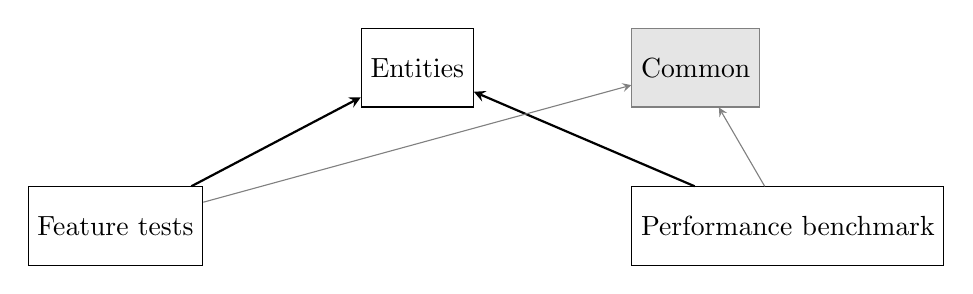
\begin{tikzpicture}[
    node distance=1cm and 2cm,
    every node/.style={draw, minimum width=1cm, minimum height=1cm, align=center},
    every path/.style={->, >=stealth},
    faded/.style={draw=gray, fill=gray!20},
    faded_arrow/.style={->, >=stealth, draw=gray}
]

  \node (E) {Entities};
  \node (C) [right=of E, faded] {Common};
  \node (FT) [below left=of E] {Feature tests};
  \node (PB) [below right=of E] {Performance benchmark};

  \draw[thick, ->, >=stealth] (FT) -- (E);
  \draw[thick, ->, >=stealth] (PB) -- (E);
  \draw[faded_arrow] (FT) -- (C);
  \draw[faded_arrow] (PB) -- (C);

\end{tikzpicture}
\end{center}

Common project is also included. It contains a single class handling loading the database connection string from a configuration file. There is no dependency between feature tests and performance tests. It could be argued that the code for queries could be extracted to a separate class to avoid duplication. But we have kept it duplicated to isolate unit tests from performance benchmarks. This structure is repeated for each of the seven frameworks we are examining. There is again no dependency between the different frameworks for isolation purposes.

\subsubsection{Technology overview}
As we have decided before implementation in \autoref{sec:dataset_database}, we are using Microsoft SQL Server database with World Wide Importers data set. The database is running in a Docker container. Base image used is \texttt{mssql/server:2022-latest}\cite{mssqlDocker} provided by Microsoft. The image imports our dataset and waits until it is ready.

The .NET tests are structured in .NET projects grouped in one solution. .NET version 8 was chosen as it is the latest LTS (long term support) version at the time of writing\cite{NETversions}. Tests were developed and run using Microsoft Visual Studio 2022, but \texttt{dotnet} CLI commands will be provided as well.

\subsubsection{Installation instructions}
The container was tested both in Docker and Podman. A Dockerfile is provided in benchmarks/Dockerfile. Container image can be built and started using the two commands below. Replace `docker` with `podman` if needed. The database will be exposed on port 1444, under username SA and password \texttt{Testingorms123}.
The third command can be used to test connection. The sqlcmd utility is available only if you have MSSQL installed locally. Otherwise, use any database management tool of your choice.

\begin{lstlisting}[language=sh]
docker build -t orm-comparison .

docker run -d --name orm-comparison -p 1444:1433 orm-comparison

sqlcmd -S 127.0.0.1,1444 -U SA -P Testingorms123 -Q "SELECT * FROM [WideWorldImporters].[Purchasing].[PurchaseOrders]"
\end{lstlisting}

To run feature unit tests, build the project in Visual Studio and then use the Test Explorer window to select and run specific tests. Alternatively, navigate to the folder with solution file and run \lstinline{dotnet test}. This will build the project, find all tests, and run them. 

To run performance benchmarks, set \texttt{BenchmarkMain} as a startup project. Right-click it in the Solution Explorer window and choose `Set as Startup project`. Make sure configuration is set to Release, not Debug. Then start the project without debugging (CTRL + F5 keys). A console window will appear. It contains instructions on how to target specific benchmarks. To run all, type in asterisk (*) and press enter. This will trigger full run, which takes approximately one hour to finish. You can switch to test configuration which does only a few number of iterations in \texttt{BenchmarkMain/Program.cs} file. What the configuration does is further explained in following sections. 

Console command for running benchmarks is \lstinline{dotnet run --configuration Release --project BenchmarkMain\BenchmarkMain.csproj}. To run with shorter test configuration append \lstinline{-- --testb} at the end of the command.


\subsubsection{Entities}
Set of classes either mirroring a database table or containing a necessary subset of properties. The columns mapped always depend on the test they are being used in. The entities are POCOs (plain old CLR objects). The term is derived from POJO (plain old Java objects). \cite{Fowler2003POJO} It refers to classes that don't inherit from any base class or interface. And they are not tied to any specific framework.

Below is an example of a POCO class for a purchase order. Visibility modifiers and some properties were omitted for readability. 

% TODO Move explanation about what entities are to earlier section/introduction

\begin{lstlisting}[language=CSharp]
class PurchaseOrder
{
    int PurchaseOrderID { get; set; }
    int SupplierID { get; set; }
    DateTime OrderDate { get; set; }
    DateTime? ExpectedDeliveryDate { get; set; }
    string? Comments { get; set; }
}
\end{lstlisting}

Some frameworks like Dapper do not need any entity mapping and simply require the properties to match selected query columns. The purchase order entity could be used to load results of a query, but the query has to return columns with matching names, data types, and nullability.

More complex frameworks that do not just perform read queries need to know how to map an entity to a database table. The corresponding table might not even exist and is generated based on the entity. Such use case is central to domain-driven development\cite{FowlerDDD}.

Entity mapping might be done in multiple ways. The simplest form is no mapping. The framework would then guess table and column names, data types, nullability, etc. from the way an entity is named and declared. Clearly, that lacks details like numeric precision, constraints, and indices.
Those details could be specified by property and class attributes. That makes them tied to an entity, which could be a problem if we want to isolate the domain model from database access. 
Mapping through code or a configuration file allows separation and can be more expressive and powerful.

To showcase different approaches to mapping, we have tried to select a different method for each framework test. Mapping is usually compiled on application startup or first query and then cached. So performance should not be affected by a choice of mapping. Dapper does not use any mapping (as it does not support any). PetaPoco and RepoDB use attributes to declare table schema and name, and in some cases column names, the rest is inferred. For those two, mapping abilities are quite limited. LINQ to DB utilizes mapping by code through builder pattern. NHibernate has its proprietary mapping through files in XML format. Both versions of Entity Framework use attribute mapping combined with mapping through code. Their attribute mapping is much more powerful than those of PetaPoco and RepoDB, but in more complex cases, mapping by code has to be supplied.

First listing below shows attribute mapping in EF Core, where attributes are placed directly above classes and properties. In the second one, part of an XML mapping file for the same entity is shown. The verbosity of the mapping is noticeable.

\begin{lstlisting}[language=CSharp,basicstyle=\ttfamily\footnotesize]
[Table("PurchaseOrders", Schema = "Purchasing")]
class PurchaseOrder
{
    [Key]
    int PurchaseOrderID { get; set; }
}
\end{lstlisting}

\begin{lstlisting}[language=xml,basicstyle=\ttfamily\footnotesize]
<?xml version="1.0" encoding="utf-8" ?>
<hibernate-mapping xmlns="urn:nhibernate-mapping-2.2" namespace="NHibernateEntities">
    <class name="NHibernateEntities.PurchaseOrder, NHibernateEntities" table="PurchaseOrders" schema="Purchasing">
        <id name="PurchaseOrderID" column="PurchaseOrderID" type="int">
            <generator class="identity" />
        </id>
        <property name="SupplierID" not-null="true" />
        <property name="OrderDate" not-null="true" />
        ...
    </class>
</hibernate-mapping>
\end{lstlisting}

\subsubsection{Feature tests}

For each query defined in \autoref{sec:selected_queries}, a unit test in the form of an isolated method was implemented. Connection and other configuration are created outside of the test in a setup part. The method executes the query and correct results are asserted. Assertion checks the amount of results and their order. Each property is tested to contain correct data to ensure mapping was done correctly.

The example below shows Query A1 (\autoref{query:a1}) implemented for Dapper. A single purchase order is retrieved based on its ID, and its properties are checked for correct values. 
\begin{lstlisting}[language=CSharp]
[Fact]
public void A1_EntityIdenticalToTable()
{
    var order = connection.QuerySingle<PurchaseOrder>(
        "SELECT * FROM WideWorldImporters.Purchasing.PurchaseOrders WHERE PurchaseOrderId = @PurchaseOrderId",
        new { PurchaseOrderId = 25 }
    );

    Assert.Multiple(() =>
    {
        Assert.Equal(25, order.PurchaseOrderID);
        Assert.Equal(12, order.SupplierID);
        Assert.Equal(new DateTime(2013, 1, 5), order.OrderDate);
        ...
    });
}
\end{lstlisting}

As decided in \autoref{sec:testing_approach} we have attempted to use LINQ query language. Where not supported we have used any available alternative that did not involve just writing raw SQL. And finally, where nothing else was possible we have used the raw alternative to have a passing test.  
%TODO mention the table that will have feature comparison

\subsubsection{Performance benchmarks}
Feature tests can assert the correctness of returned results and overall functionality. But their execution time can greatly vary. There can be some overhead, coming from test initialization or assertions. The system the benchmarks are running on can also impact results.

To solve these problems we have used BenchmarkDotNet library\cite{BenchmarkDotNet}. It allows writing benchmark methods very similar to unit tests. In fact, they are completely identical to unit tests, the only differences are missing assertions and a different method attribute. It allows us to ``transform methods into benchmarks, track their performance, and share reproducible measurement experiments`` \cite{BenchmarkDotNet}. Work with the library was quite easy, it is very configurable and easy to run. 

It runs benchmark for each method multiple times. It starts with a few iterations which will not be included in the results. The first few ensure just-in-time compilation has taken effect, then multiple iterations without actually running the method code are started to compile overhead. The overhead is removed from the results, ensuring reliability. 


According to BenchmarkDotNet documentation\cite{BenchmarkDotNetHow} a single benchmark run consists of the following stages.
\begin{itemize}
    \item OverheadJitting - Measures benchmarking infrastructure compilation.
    \item WorkloadJitting - Measures benchmark method compilation.
    \item WorkloadPilot - Selects best iteration count based on heuristics.
    \item WorkloadWarmup - Runs several iterations before measuring to ensure factors like CPU caching or branch prediction are optimized.
    \item WorkloadActual - Actual measurements
    \item WorkloadResult - Result calculated from the actual run without the overhead.
\end{itemize}

After the benchmark run finishes, results and run log can be found in:

\smallskip
\noindent\path{benchmarks/BenchmarkMain/bin/Release/net8.0/BenchmarkDotNet.Artifacts}

\smallskip
The referenced run results are copied to:

\smallskip
\noindent\path{benchmarks/results/joined}

\smallskip
Notable result files include:
\begin{itemize}
    \item \path{BenchmarkRun-joined-2025-03-06-16-10-18-report.csv}\\
    Measurements of all benchmarks in CSV format.

    \item \path{BenchmarkRun-joined-2025-03-06-16-10-18-report.html}\\
    Summary table of all benchmarks (HTML format).

    \item \path{BenchmarkRun-joined-2025-03-06-16-10-18-report-github.md}\\
    Summary table of all benchmarks (Markdown format suitable for GitHub).

    \item \path{BenchmarkRun-joined-2025-03-06-16-10-18-measurements.csv}\\
    Detailed measurements of every single iteration of each benchmark.
\end{itemize}

\subsection{Results interpretation}
Results are accompanied by tables showing results across all test cases. 

\autoref{tab:feature_comp} summarizes feature test outcomes. The base result indicates if the query could be expressed within each framework (Y = yes, N = no). Outcomes are categorized as:
\begin{itemize}
    \item \textbf{Y LINQ}: LINQ fully supported.
    \item \textbf{Y lambda expr.}: Supported using lambda expressions, less expressive than LINQ.
    \item \textbf{Y raw SQL}: Query had to be written directly in SQL, either in string or using a builder.
    \item \textbf{N manually in memory}: Query required manual post-computation in memory.
    \item \textbf{N custom JSON parsing/converter}: JSON could not be queried and had to be parsed in memory.
    \item \textbf{N error}: Query failed with exception that could not be fixed. 
\end{itemize}
The negative results are discussed in detail further in the text.

\autoref{tab:benchmark_results_time} presents measured execution time (in microseconds). \autoref{tab:benchmark_results_memory} presents allocated memory during the run of the benchmark. Reported numbers in text will be rounded to the nearest integer.

Performance tests have to be considered in the context of the feature test results. It was not possible to write all tests in the same way across all frameworks. In some cases, pure ADO.NET queries were used when the framework failed entirely. Additionally, some queries required additional processing in memory, significantly affecting memory usage. These anomalies will be explicitly noted.

Certain frameworks cannot log generated SQL statements to console or file. For those, SQL Server Profiler\cite{sqlProfiler} was used. It allows capturing of any event happening in the SQL Server database, including incoming SQL queries. That makes us able to inspect the raw query after it leaves our application and the frameworks can make no further edits to it.

\subsubsection{Benchmark execution environment}
Performance benchmarks were executed on a single computer configured for the highest performance:
\begin{itemize}
    \item Windows 11, AMD Ryzen 5 5600H CPU (6 physical cores, 12 logical)
    \item .NET SDK version: 9.0.101
    \item Execution framework: BenchmarkDotNet v0.14.0
    \item Runtime: .NET 8.0.11, X64 architecture, RyuJIT AVX2
\end{itemize}

\subsubsection{A - Entity projection}
The first three queries \hyperref[query:a1]{A1}, \hyperref[query:a2]{A2} and \hyperref[query:a3]{A3} fetched and reshaped one database record successfully across all frameworks. Macro ORMs (EF, NHibernate) used LINQ \texttt{Select} method. Micro ORMs utilized projection in SQL query directly.
Minor performance differences appeared, macro ORMs were slightly slower. Notably, NHibernate and EF6 showed significant 2 to 10 times memory allocation spikes. EF Core is clearly optimized in this area.

Query \hyperref[query:a4]{A4} tested loading results of a stored procedure. The volume of data is approximately 60,000 rows. The stored procedure in our test dataset returns column names with spaces. Which is definitely unusual, but we would not expect a framework to completely fail. Dapper, PetaPoco, RepoDB, linq2db, and EF Core succeeded using raw SQL. Memory allocation varied significantly for those (16 MB to 29 MB). No major difference in the executed query was found using SQL Server Profiler.

NHibernate failed on an internal error. The error message \texttt{Could not find a setter for property 'WWI Order ID' in class 'System.RuntimeType'} suggests the framework failed to fill an internal memory representation of the entity. A workaround using a hash table increased both time and memory significantly.

EF6 completely failed, with no viable workaround this time. The test uses a pure ADO.NET connection, with no EF6 features whatsoever. We consider the test failed and the measurements are not relevant for our comparison.

\subsubsection{B - Selection}
All selection queries \hyperref[query:b1]{B1} - \hyperref[query:b6]{B6} passed in terms of features. As expected, Dapper and PetaPoco required explicit SQL, while macro ORMs supported LINQ. Memory usage varied significantly, particularly for NHibernate and EF6.

Query \hyperref[query:b1]{B1}, which returns 5 records, showed macro ORMs allocating significantly more memory (NHibernate 49 KB, EF6 102 KB) compared to Dapper (9 KB) or PetaPoco (14 KB). Query \hyperref[query:b2]{B2}, returning thousands of records, again showed NHibernate and E6 taking drastically more time and memory (7 and 16 times more), even though generated SQL queries were identical.

Query \hyperref[query:b3]{B3} showed unexpectedly slower performance from Dapper, PetaPoco, and RepoDB. There is a difference in the query. In Dapper and PetaPoco, where SQL is written by us, we used \texttt{BETWEEN} condition for selecting a date range. Other ORMs broke this condition down into two operators ($\leq$ and $\geq$). But RepoDB does not use \texttt{BETWEEN}, hinting that this had no impact.

Queries \hyperref[query:b4]{B4}, \hyperref[query:b5]{B5}, and \hyperref[query:b6]{B6} had generally consistent execution times across all frameworks. But NHibernate and EF6 showed consistently elevated memory allocation. Interestingly, in some cases, Dapper showed higher memory usage compared to PetaPoco, indicating differences in internal memory optimization. 

\subsubsection{C - Aggregation}
Aggregation tests \hyperref[query:c1]{C1} - \hyperref[query:c3]{C3} tested handling of groupings and aggregate functions. RepoDB lacked support for \texttt{group by} operation in query C, failing the test entirely. NHibernate and EF6 have approximately a 4 and 10 times memory consumption increase, respectively, although execution times remain comparable. 

\hyperref[query:c2]{C2} showed consistent performance and memory usage across frameworks. However, in \hyperref[query:c3]{C3}, RepoDB incorrectly handled a multiplication when using its \texttt{Sum} function. It omitted part of the multiplication inside the \texttt{sum} aggregation function, returning incorrect results. We had to use a raw SQL query instead. The measured time is consistent across all frameworks. The returned result is just one number and we can see some slight increase in memory consumption for the macro ORMs.

In summary, RepoDB did not handle aggregation functions well. EF Core is showing its optimization by approaching the results of micro ORMs.

\subsubsection{D - Relations}
This group evaluates how effectively ORMs handle relational data - specifically one-to-many, many-to-many, and optional one-to-many relationships. Macro ORMs managed to automatically retrieve related entities once mapping was correctly defined. On the other hand, micro ORMs generally required raw SQL data fetching and in-memory grouping. Parent-child pairs were fetched individually before grouping them using dictionaries.

In query \hyperref[query:d1]{D1} one parent with a few children was fetched. NHibernate and EF6 again showed increased memory usage, around 4 to 6 times higher.

Query \hyperref[query:d2]{D2} examined a dense many-to-many relationship involving 227 entities on one side and 10 on the other. RepoDB passed the other two queries, but this one had to be done in memory. linq2db required an explicit join entity, while the other macro ORMs directly mapped child collections within parent entities.

Query \hyperref[query:d3]{D3} tested an optional one-to-many relationship. Linq2db had the best results, using separate queries for parents and children without any optimization enabled. Surprisingly, EF Core performed the worst, taking 2548 ms compared to Dapper's 187 ms. This inefficiency remained even after experimenting with different tracking settings and the split query feature. When running the raw generated query directly, it was executed in less than 200 ms.

We could see EF Core performing well among the previous categories, but it is really slow when it comes to relationships. Raw SQL combined with manual memory grouping or using linq2db seems to be the best option for queries over relationships.

\subsubsection{E - Result modification}
Queries \hyperref[query:e1]{E1} and \hyperref[query:e2]{E2} tested column sorting and distinct results. All ORMs passed these tests with no significant difference. Only NHibernate and EF6 showed increased memory consumption. 

\subsubsection{F - Querying JSON}
These tests targeted JSON querying capabilities within a string column. Only EF Core provides full LINQ integration. Other frameworks required raw SQL with MSSQL JSON functions and subsequent manual JSON parsing.

Both queries \hyperref[query:f1]{F1} and \hyperref[query:f2]{F2} showed similar execution times. Allocated memory differs slightly, mainly for NHibernate and EF6 once again. Interestingly, PetaPoco consumed over twice the memory of Dapper despite identical queries.

\subsubsection{G - Set operations}
Query \hyperref[query:g1]{G1} tested union and \hyperref[query:g2]{G2} intersection. Macro ORMs took roughly double the time. However, considering the small result set ($<$ 10), the variation can likely be attributed to framework overhead.

\subsubsection{H - Querying metadata}
The final test \hyperref[query:h1]{H1} queried table metadata, specifically the data type of a single column. No ORM had native support, requiring a raw SQL query to \texttt{INFORMATION\_SCHEMA.COLUMNS} table. There are small differences, we can likely attribute them to framework overhead.

\subsubsection{Summary of findings}
Performance and feature test results clearly differ between micro and macro ORMs. Macro ORMs (NHibernate, EF6, EF Core) offer richer features and better abstractions. But that comes at the cost of increased execution time and memory overhead, particularly noticeable in the older EF6 and NHibernate. EF Core consistently demonstrates strong optimizations, often competing with micro ORMs. However, it notably struggles with relational queries. 

Micro ORMs (Dapper and PetaPoco) require manual SQL handling, resulting in minimal time and memory overhead. They generally handle their limited features well. Linq2db strikes a good balance between speed and abstraction over SQL. It handles complex relationships notably well. Lastly, RepoDB stands at a strange middle ground, neither being best in any category nor offering a wide range of features.

Considering our test results alongside other factors---our previous findings about popularity, update frequency and overall functionality---EF Core emerges as the best choice for most applications. It has the widest feature set with solid optimizations. However, when performance is the critical factor, choosing raw queries with Dapper might be a better alternative.

%\clearpage
\afterpage{
\begin{landscape}
%If the table is too wide, replace \begin{table}[!htp]...\end{table} with
%\begin{adjustwidth}{-2.5 cm}{-2.5 cm}\centering\begin{threeparttable}[!htb]...\end{threeparttable}\end{adjustwidth}
%\begin{adjustwidth}{-2.5 cm}{-2.5 cm}
\begin{table}[htp]
\centering
\caption{Feature comparison}
\label{tab:feature_comp}
\scriptsize
\begin{threeparttable}[!htb]
\def\arraystretch{1.25}
\begin{tabular}{
>{\raggedright\arraybackslash}p{50.00mm}
>{\raggedright\arraybackslash}p{20.00mm}
>{\raggedright\arraybackslash}p{20.00mm}
>{\raggedright\arraybackslash}p{20.00mm}
>{\raggedright\arraybackslash}p{20.00mm}
>{\raggedright\arraybackslash}p{20.00mm}
>{\raggedright\arraybackslash}p{20.00mm}
>{\raggedright\arraybackslash}p{20.00mm}
>{\raggedright\arraybackslash}p{20.00mm}
}
\toprule
\textbf{Benchmark Name} & \textbf{Dapper} & \textbf{PetaPoco} & \textbf{RepoDB} & \textbf{linq2db} & \textbf{NHibernate} & \textbf{EF6} & \textbf{EF Core} \\
\midrule
A1\_EntityIdenticalToTable &Y raw SQL &Y raw SQL &\cellcolor[HTML]{d9ead3}Y lambda expr. &\cellcolor[HTML]{b7e1cd}Y LINQ &\cellcolor[HTML]{b7e1cd}Y LINQ &\cellcolor[HTML]{b7e1cd}Y LINQ &\cellcolor[HTML]{b7e1cd}Y LINQ \\
A2\_LimitedEntity &Y raw SQL &Y raw SQL &\cellcolor[HTML]{d9ead3}Y lambda expr. &\cellcolor[HTML]{b7e1cd}Y LINQ &\cellcolor[HTML]{b7e1cd}Y LINQ &\cellcolor[HTML]{b7e1cd}Y LINQ &\cellcolor[HTML]{b7e1cd}Y LINQ \\
A3\_MultipleEntitiesFromOneResult &Y raw SQL &Y raw SQL &\cellcolor[HTML]{d9ead3}Y lambda expr. &\cellcolor[HTML]{b7e1cd}Y LINQ &\cellcolor[HTML]{b7e1cd}Y LINQ &\cellcolor[HTML]{b7e1cd}Y LINQ &\cellcolor[HTML]{b7e1cd}Y LINQ \\
A4\_StoredProcedureToEntity &Y raw SQL &Y raw SQL &Y raw SQL &Y raw SQL &\cellcolor[HTML]{ea9999}N error &\cellcolor[HTML]{ea9999}N error &Y raw SQL \\
B1\_SelectionOverIndexedColumn &Y raw SQL &Y raw SQL &\cellcolor[HTML]{d9ead3}Y lambda expr. &\cellcolor[HTML]{b7e1cd}Y LINQ &\cellcolor[HTML]{b7e1cd}Y LINQ &\cellcolor[HTML]{b7e1cd}Y LINQ &\cellcolor[HTML]{b7e1cd}Y LINQ \\
B2\_SelectionOverNonIndexedColumn &Y raw SQL &Y raw SQL &\cellcolor[HTML]{d9ead3}Y lambda expr. &\cellcolor[HTML]{b7e1cd}Y LINQ &\cellcolor[HTML]{b7e1cd}Y LINQ &\cellcolor[HTML]{b7e1cd}Y LINQ &\cellcolor[HTML]{b7e1cd}Y LINQ \\
B3\_RangeQuery &Y raw SQL &Y raw SQL &\cellcolor[HTML]{d9ead3}Y lambda expr. &\cellcolor[HTML]{b7e1cd}Y LINQ &\cellcolor[HTML]{b7e1cd}Y LINQ &\cellcolor[HTML]{b7e1cd}Y LINQ &\cellcolor[HTML]{b7e1cd}Y LINQ \\
B4\_InQuery &Y raw SQL &Y raw SQL &\cellcolor[HTML]{d9ead3}Y lambda expr. &\cellcolor[HTML]{b7e1cd}Y LINQ &\cellcolor[HTML]{b7e1cd}Y LINQ &\cellcolor[HTML]{b7e1cd}Y LINQ &\cellcolor[HTML]{b7e1cd}Y LINQ \\
B5\_TextSearch &Y raw SQL &Y raw SQL &\cellcolor[HTML]{d9ead3}Y lambda expr. &\cellcolor[HTML]{b7e1cd}Y LINQ &\cellcolor[HTML]{b7e1cd}Y LINQ &\cellcolor[HTML]{b7e1cd}Y LINQ &\cellcolor[HTML]{b7e1cd}Y LINQ \\
B6\_PagingQuery &Y raw SQL &Y raw SQL &\cellcolor[HTML]{d9ead3}Y lambda expr. &\cellcolor[HTML]{b7e1cd}Y LINQ &\cellcolor[HTML]{b7e1cd}Y LINQ &\cellcolor[HTML]{b7e1cd}Y LINQ &\cellcolor[HTML]{b7e1cd}Y LINQ \\
C1\_AggregationCount &Y raw SQL &Y raw SQL &\cellcolor[HTML]{f4cccc}N manually in memory &\cellcolor[HTML]{b7e1cd}Y LINQ &\cellcolor[HTML]{b7e1cd}Y LINQ &\cellcolor[HTML]{b7e1cd}Y LINQ &\cellcolor[HTML]{b7e1cd}Y LINQ \\
C2\_AggregationMax &Y raw SQL &Y raw SQL &\cellcolor[HTML]{d9ead3}Y lambda expr. &\cellcolor[HTML]{b7e1cd}Y LINQ &\cellcolor[HTML]{b7e1cd}Y LINQ &\cellcolor[HTML]{b7e1cd}Y LINQ &\cellcolor[HTML]{b7e1cd}Y LINQ \\
C3\_AggregationSum &Y raw SQL &Y raw SQL &Y raw SQL &\cellcolor[HTML]{b7e1cd}Y LINQ &\cellcolor[HTML]{b7e1cd}Y LINQ &\cellcolor[HTML]{b7e1cd}Y LINQ &\cellcolor[HTML]{b7e1cd}Y LINQ \\
D1\_OneToManyRelationship &\cellcolor[HTML]{f4cccc}N manually in memory &\cellcolor[HTML]{f4cccc}N manually in memory &\cellcolor[HTML]{d9ead3}Y lambda expr. &\cellcolor[HTML]{b7e1cd}Y LINQ + mapping &\cellcolor[HTML]{b7e1cd}Y LINQ + mapping &\cellcolor[HTML]{b7e1cd}Y LINQ + mapping &\cellcolor[HTML]{b7e1cd}Y LINQ + mapping \\
D2\_ManyToManyRelationship &\cellcolor[HTML]{f4cccc}N manually in memory &\cellcolor[HTML]{f4cccc}N manually in memory &\cellcolor[HTML]{f4cccc}N manually in memory &\cellcolor[HTML]{b7e1cd}Y LINQ + mapping, join entity &\cellcolor[HTML]{b7e1cd}Y LINQ + mapping &\cellcolor[HTML]{b7e1cd}Y LINQ + mapping &\cellcolor[HTML]{b7e1cd}Y LINQ + mapping \\
D3\_OptionalRelationship &\cellcolor[HTML]{f4cccc}N manually in memory &\cellcolor[HTML]{f4cccc}N manually in memory &\cellcolor[HTML]{d9ead3}Y lambda expr. &\cellcolor[HTML]{b7e1cd}Y LINQ + mapping &\cellcolor[HTML]{b7e1cd}Y LINQ + mapping &\cellcolor[HTML]{b7e1cd}Y LINQ + mapping &\cellcolor[HTML]{b7e1cd}Y LINQ + mapping \\
E1\_ColumnSorting &Y raw SQL &Y raw SQL &\cellcolor[HTML]{d9ead3}Y lambda expr. &\cellcolor[HTML]{b7e1cd}Y LINQ &\cellcolor[HTML]{b7e1cd}Y LINQ &\cellcolor[HTML]{b7e1cd}Y LINQ &\cellcolor[HTML]{b7e1cd}Y LINQ \\
E2\_Distinct &Y raw SQL &Y raw SQL &Y raw SQL &\cellcolor[HTML]{b7e1cd}Y LINQ &\cellcolor[HTML]{b7e1cd}Y LINQ &\cellcolor[HTML]{b7e1cd}Y LINQ &\cellcolor[HTML]{b7e1cd}Y LINQ \\
F1\_NestedJSONQuery &\cellcolor[HTML]{f4cccc}N custom JSON parsing &\cellcolor[HTML]{f4cccc}N custom JSON parsing &\cellcolor[HTML]{f4cccc}N custom JSON parsing &\cellcolor[HTML]{f4cccc}N custom converter &\cellcolor[HTML]{f4cccc}N custom JSON parsing &\cellcolor[HTML]{f4cccc}N custom JSON parsing &\cellcolor[HTML]{b7e1cd}Y LINQ \\
F2\_JSONArrayQuery &\cellcolor[HTML]{f4cccc}N custom JSON parsing &\cellcolor[HTML]{f4cccc}N custom JSON parsing &\cellcolor[HTML]{f4cccc}N custom JSON parsing &\cellcolor[HTML]{f4cccc}N custom converter &\cellcolor[HTML]{f4cccc}N custom JSON parsing &\cellcolor[HTML]{f4cccc}N custom JSON parsing &\cellcolor[HTML]{b7e1cd}Y LINQ \\
G1\_Union &Y raw SQL &Y raw SQL &Y raw SQL &\cellcolor[HTML]{b7e1cd}Y LINQ &\cellcolor[HTML]{b7e1cd}Y LINQ &\cellcolor[HTML]{b7e1cd}Y LINQ &\cellcolor[HTML]{b7e1cd}Y LINQ \\
G2\_Intersection &Y raw SQL &Y raw SQL &Y raw SQL &\cellcolor[HTML]{b7e1cd}Y LINQ &\cellcolor[HTML]{b7e1cd}Y LINQ &\cellcolor[HTML]{b7e1cd}Y LINQ &\cellcolor[HTML]{b7e1cd}Y LINQ \\
H1\_Metadata &Y raw SQL &Y raw SQL &Y raw SQL &Y raw SQL &Y raw SQL &Y raw SQL &Y raw SQL \\
\bottomrule
\end{tabular}
\end{threeparttable}
\end{table}
%\end{adjustwidth}
\end{landscape}
}


\clearpage
\begin{landscape}
\begin{table}
\centering
\caption{Performance benchmark results - Mean time (\unit{\micro\second})}
\label{tab:benchmark_results_time}
\scriptsize
\def\arraystretch{1.35}
\begin{tabular}{
>{\raggedright\arraybackslash}p{50.00mm}
>{\raggedleft\arraybackslash}p{20.00mm}
>{\raggedleft\arraybackslash}p{20.00mm}
>{\raggedleft\arraybackslash}p{20.00mm}
>{\raggedleft\arraybackslash}p{20.00mm}
>{\raggedleft\arraybackslash}p{20.00mm}
>{\raggedleft\arraybackslash}p{20.00mm}
>{\raggedleft\arraybackslash}p{20.00mm}
>{\raggedleft\arraybackslash}p{20.00mm}
}
\toprule
\textbf{Namespace} &    \textbf{Dapper} &  \textbf{PetaPoco} &    \textbf{RepoDB} &   \textbf{Linq2db} &  \textbf{NHibernate} &        \textbf{EF6} &     \textbf{EFCore} \\
\midrule
A1\_EntityIdenticalToTable        &      750 &      722 &      748 &      839 &        742 &        854 &        809 \\
A2\_LimitedEntity                 &      718 &      726 &      735 &      858 &        958 &        882 &        799 \\
A3\_MultipleEntitiesFromOneResult &      736 &      736 &      745 &      898 &      1 001 &        945 &        832 \\
A4\_StoredProcedureToEntity       &  523 239 &  505 967 &  523 242 &  519 491 &    621 739 &    514 077 &    521 573 \\
B1\_SelectionOverIndexedColumn    &      744 &      759 &      762 &      868 &        817 &        905 &        806 \\
B2\_SelectionOverNonIndexedColumn &   43 612 &   41 100 &   43 052 &   43 708 &     86 419 &    125 169 &     48 016 \\
B3\_RangeQuery                    &   30 393 &   29 935 &   30 746 &   21 909 &     22 289 &     22 823 &     21 102 \\
B4\_InQuery                       &      856 &      855 &      876 &      954 &        945 &      1 408 &      1 147 \\
B5\_TextSearch                    &  747 728 &  747 721 &  745 551 &  745 319 &    746 464 &    746 264 &    744 754 \\
B6\_PagingQuery                   &    1 327 &    1 314 &    1 556 &    1 458 &      1 447 &      1 710 &      1 406 \\
C1\_AggregationCount              &   35 006 &   35 289 &  377 349 &   35 372 &     35 553 &     35 364 &     35 286 \\
C2\_AggregationMax                &    1 240 &    1 227 &    1 264 &    1 380 &      1 291 &      1 366 &      1 304 \\
C3\_AggregationSum                &   86 499 &   85 944 &   86 899 &   86 145 &     75 137 &     69 827 &     87 825 \\
D1\_OneToManyRelationship         &      781 &      770 &      806 &    2 997 &      1 042 &      1 581 &        895 \\
D2\_ManyToManyRelationship        &    4 584 &    4 480 &    6 031 &    9 383 &      5 940 &      6 913 &     14 964 \\
D3\_OptionalRelationship          &  187 693 &  172 030 &  393 631 &   91 326 &    533 489 &  1 993 146 &  2 548 411 \\
E1\_ColumnSorting                 &    4 725 &    4 622 &    4 963 &    4 845 &      6 316 &      6 204 &      4 885 \\
E2\_Distinct                      &    2 181 &    2 148 &    2 180 &    2 374 &      2 229 &      2 340 &      2 270 \\
F1\_JSONObjectQuery               &    1 459 &    1 478 &    1 457 &    1 552 &      1 494 &      1 490 &      1 544 \\
F2\_JSONArrayQuery                &    1 723 &    1 718 &    1 732 &    1 795 &      1 761 &      1 771 &      1 839 \\
G1\_Union                         &      728 &      715 &      723 &    1 580 &      1 538 &      1 613 &      1 561 \\
G2\_Intersection                  &      739 &      718 &      730 &    1 596 &      1 534 &      1 622 &      1 566 \\
H1\_Metadata                      &      851 &      843 &      844 &      925 &        866 &        899 &        814 \\
\bottomrule
\end{tabular}
\end{table}
\end{landscape}

\clearpage
\begin{landscape}
\begin{table}
\centering
\caption{Performance benchmark results - Allocated memory (KB)}
\label{tab:benchmark_results_memory}
\scriptsize
\def\arraystretch{1.35}
\begin{tabular}{
>{\raggedright\arraybackslash}p{50.00mm}
>{\raggedleft\arraybackslash}p{20.00mm}
>{\raggedleft\arraybackslash}p{20.00mm}
>{\raggedleft\arraybackslash}p{20.00mm}
>{\raggedleft\arraybackslash}p{20.00mm}
>{\raggedleft\arraybackslash}p{20.00mm}
>{\raggedleft\arraybackslash}p{20.00mm}
>{\raggedleft\arraybackslash}p{20.00mm}
>{\raggedleft\arraybackslash}p{20.00mm}
}
\toprule
\textbf{Namespace}                         &    \textbf{Dapper} &  \textbf{PetaPoco} &    \textbf{RepoDB} &   \textbf{Linq2db} & \textbf{NHibernate} &      \textbf{EF6} &    \textbf{EFCore} \\
\midrule
A1\_EntityIdenticalToTable        &      6.24 &     7.99 &      8.77 &     12.74 &      36.06 &    90.43 &    14.49 \\
A2\_LimitedEntity                 &      4.74 &     9.64 &      7.99 &     18.25 &      50.70 &   115.18 &    16.11 \\
A3\_MultipleEntitiesFromOneResult &      7.28 &    13.03 &     10.38 &     27.74 &      84.00 &   211.61 &    25.85 \\
A4\_StoredProcedureToEntity       &  24294.84 & 16490.15 &  17007.14 &  16490.93 &   91569.96 & 35270.68 & 29008.69 \\
B1\_SelectionOverIndexedColumn    &      8.63 &    14.30 &      9.79 &     14.63 &      49.46 &   102.35 &    12.88 \\
B2\_SelectionOverNonIndexedColumn &   7112.75 &  3308.54 &   3410.07 &   3314.16 &   21371.02 & 50014.45 &  5847.86 \\
B3\_RangeQuery                    &    989.93 &   468.38 &    480.34 &    475.55 &    3048.82 &  6747.98 &   819.92 \\
B4\_InQuery                       &     16.92 &    20.34 &     16.64 &     19.58 &      87.42 &   354.18 &    19.85 \\
B5\_TextSearch                    &   1169.29 &   587.24 &    599.41 &    592.78 &    3472.99 &  8113.77 &   979.42 \\
B6\_PagingQuery                   &     32.59 &    25.06 &     18.25 &     26.58 &     128.29 &   265.26 &    40.52 \\
C1\_AggregationCount              &      2.75 &     8.79 &  59994.30 &     12.46 &      41.75 &   117.99 &    12.04 \\
C2\_AggregationMax                &      1.97 &     4.19 &      1.77 &      8.12 &      23.06 &    77.09 &     5.69 \\
C3\_AggregationSum                &      2.09 &     4.41 &      1.35 &      9.25 &      25.31 &    81.72 &     6.85 \\
D1\_OneToManyRelationship         &     16.46 &    17.94 &     20.23 &     24.58 &      88.71 &   115.27 &    26.44 \\
D2\_ManyToManyRelationship        &    433.35 &   381.13 &    854.28 &    352.15 &    1162.43 &  1395.95 &  2555.79 \\
D3\_OptionalRelationship          &  40923.17 & 24909.64 &  20945.39 &   9083.71 &  144094.98 &278566.55 &175866.23 \\
E1\_ColumnSorting                 &    349.40 &   156.96 &    162.62 &    162.54 &    1354.02 &  2000.95 &   348.07 \\
E2\_Distinct                      &      2.42 &     4.78 &      1.66 &      9.34 &      23.72 &    76.19 &     8.54 \\
F1\_JSONObjectQuery               &     21.71 &    45.25 &     31.82 &     27.09 &      86.13 &    73.38 &    51.68 \\
F2\_JSONArrayQuery                &      6.04 &    18.12 &      8.25 &     11.30 &      74.31 &    57.24 &    16.86 \\
G1\_Union                         &      2.39 &     3.45 &      1.40 &     18.03 &      60.07 &   136.10 &    20.35 \\
G2\_Intersection                  &      2.17 &     3.25 &      1.30 &     17.91 &      61.36 &   135.98 &    21.73 \\
H1\_Metadata                      &      1.98 &     5.10 &      1.21 &      5.61 &      35.53 &    46.52 &    10.99 \\
\bottomrule
\end{tabular}
\end{table}
\end{landscape}
